% !TEX program = xelatex
% 智舆——AI城市舆情态势监测感知与决策推演系统 项目策划书
\documentclass[12pt,a4paper,fontset=windows,AutoFakeBold=2]{ctexart}

% 宏包引入
\usepackage{geometry}
\usepackage{graphicx}
\usepackage{amsmath}
\usepackage{amssymb}
\usepackage{booktabs}
\usepackage{longtable}
\usepackage{array}
\usepackage{multirow}
\usepackage{xcolor}
\usepackage{hyperref}
\usepackage{listings}
\usepackage{fancyhdr}
\usepackage{titlesec}
\usepackage{enumitem}
\usepackage{float}
\usepackage{subcaption}
\usepackage{tcolorbox}
\usepackage{setspace}

% 页面设置
\geometry{left=2.5cm,right=2.5cm,top=3cm,bottom=2.5cm,headheight=28pt}

% ==================== 字体设置(符合模板要求) ====================
% ctex 内置字体命令: \songti, \heiti, \kaishu, \fangsong, \yahei
% fontset=windows 已自动配置中文字体

% 字号定义(LaTeX标准字号对照)
% 初号 = 42pt, 二号 = 22pt, 三号 = 16pt, 四号 = 14pt, 小四 = 12pt
\newcommand{\chuhao}{\fontsize{42pt}{50pt}\selectfont}
\newcommand{\erhao}{\fontsize{22pt}{26pt}\selectfont}
\newcommand{\sanhao}{\fontsize{16pt}{20pt}\selectfont}
\newcommand{\sihao}{\fontsize{14pt}{18pt}\selectfont}
\newcommand{\xiaosi}{\fontsize{12pt}{15pt}\selectfont}

% 颜色定义
\definecolor{primaryblue}{RGB}{0,82,155}
\definecolor{accentcyan}{RGB}{6,182,212}
\definecolor{codebg}{RGB}{245,245,245}

% 超链接设置
\hypersetup{colorlinks=true,linkcolor=primaryblue,urlcolor=accentcyan}

% 代码样式
\lstset{basicstyle=\small\ttfamily,backgroundcolor=\color{codebg},frame=single,breaklines=true}

% 标题格式(符合模板要求)
% 章标题:微软雅黑 三号 加粗
\titleformat{\section}{\yahei\sanhao\color{primaryblue}}{第\chinese{section}章}{1em}{}
% 节标题:微软雅黑 四号 加粗
\titleformat{\subsection}{\yahei\sihao}{\thesubsection}{1em}{}
% 小节标题:微软雅黑 小四 加粗
\titleformat{\subsubsection}{\yahei\xiaosi}{\thesubsubsection}{1em}{}

% 正文字体:宋体 四号(在document开始时设置)
\AtBeginDocument{\songti\sihao}

% 页眉页脚
\pagestyle{fancy}
\fancyhf{}
\renewcommand{\headrulewidth}{0.4pt}
\fancyhead[L]{\raisebox{-0.3\height}{\includegraphics[height=0.8cm]{picture/logo.png}}\hspace{0.3cm}\small 信阳学院首届"数智讯飞杯"AI+创新应用大赛}
\fancyhead[R]{\small 项目策划书}
\fancyfoot[C]{\thepage}
\setlength{\headheight}{28pt}

% 图表说明框
\newtcolorbox{figurebox}{colback=blue!5,colframe=accentcyan,boxrule=1pt,arc=3pt}

% 目录格式:宋体 二号
\usepackage{tocloft}
\renewcommand{\cfttoctitlefont}{\songti\erhao\bfseries}
\renewcommand{\cftaftertoctitle}{\hfill}
\renewcommand{\cftsecfont}{\songti\sihao}
\renewcommand{\cftsubsecfont}{\songti\xiaosi}

% 表格列类型
\newcolumntype{L}[1]{>{\raggedright\arraybackslash}p{#1}}
\newcolumntype{C}[1]{>{\centering\arraybackslash}p{#1}}

% 行间距
\setstretch{1.5}

\begin{document}

% 封面
% 封面
\begin{titlepage}
    \centering
    

    
    % 学校名称 - 微软雅黑 二号
    {\yahei\erhao\bfseries 信阳学院}
    
    \vspace{0.3cm}
    
    % 大赛名称 - 微软雅黑 二号
    {\yahei\erhao\bfseries 首届'数智讯飞杯'AI+创新应用大赛}
    
    \vspace{1cm}
    
    % 项目名称 - 仿宋 红色 括号
    {\fangsong\sanhao\color{red} (智舆——AI城市舆情态势监测感知与决策推演系统)}
    
    % 顶部Logo

    \vspace{0.5cm}
    
    \includegraphics[height=4cm]{picture/logo.png}
    
    \vspace{0.5cm}
    
    % 策划书 - 黑体 加粗 初号 竖排
    {\heiti\bfseries\chuhao 策}
    
    \vspace{0.8cm}
    \vspace{0.8cm}
    
    {\heiti\bfseries\chuhao 划}
    
    \vspace{0.8cm}
    \vspace{0.8cm}
    
    {\heiti\bfseries\chuhao 书}
    
    \vfill
    
    % 底部信息 - 微软雅黑 四号
    \begin{flushleft}
        \hspace{3cm}
        \begin{tabular}{ll}
            {\yahei\sihao\bfseries 项目名称:} & {\yahei\sihao 智舆——AI城市舆情态势监测感知与决策推演系统} \\[1em]
            {\yahei\sihao\bfseries 团队名称:} & {\yahei\sihao X.X小队} \\[1em]
            {\yahei\sihao\bfseries 团队成员:} & {\yahei\sihao 安思言 \ 李智康 \ 叶照扬 \ 王佳蕾 \ 李欣然 \ 程文飞} \\[1em]
        \end{tabular}
    \end{flushleft}
    
    
\end{titlepage}


% 目录
\newpage
\tableofcontents
\newpage

% 各章节
% 第一章 项目概述
\section{项目概述}

\subsection{项目简介}

\textbf{智舆}是一款面向城市治理的AI智慧舆情态势监测感知与决策推演系统,旨在通过人工智能技术赋能传统舆情监测,构建集\textbf{数据采集、智能分析、3D可视化展示、走向预测、决策模拟}于一体的综合性平台。

系统核心价值在于:\textbf{让城市管理者"看得见"舆情态势、"听得懂"民意诉求、"想得清"发展走向、"做得好"科学决策}。

本项目采用\textbf{讯飞星火4.0大模型}作为核心AI分析引擎,结合\textbf{高德地图3D可视化}、\textbf{多Agent决策推演}、\textbf{城市模型矩阵}、\textbf{语音交互播报}等创新技术,实现从舆情监测到辅助决策的全流程智能化。系统支持\textbf{全国-省份-地级-县级}四级区域穿透分析,可根据文字、图片、视频等多模态舆情内容AI生成现场3D模型,并通过决策模拟功能帮助用户预判不同应对策略的效果。创新性地构建\textbf{城市模型矩阵},基于LoRA微调技术为不同城市/省份训练专属适配器,实现本地化舆情精准分析。

项目首期聚焦\textbf{信阳市}场景落地,逐步扩展至河南省乃至全国城市,为政府、企业、个人提供差异化的舆情智慧服务。

\subsection{项目背景}

\subsubsection{政策背景}

\textbf{国家层面}高度重视智慧城市与数字政府建设。2025年10月,国家发改委等五部门联合印发《深化智慧城市发展推进全域数字化转型行动计划》,明确提出到2027年底建成50个以上全域数字化转型城市。《国务院关于加强数字政府建设的指导意见》确立了到2025年政府数字化履职能力框架基本形成的目标。

\textbf{河南省层面},《河南省深化智慧城市发展推进城市全域数字化转型实施方案(2025-2027年)》提出打造3-5个国内一流的综合型城市全域数字化转型标杆。《河南省支持人工智能产业生态发展若干政策措施》提供真金白银支持:对通过国家生成式AI模型备案的企业给予100万元资金支持,设立30亿元人工智能产业基金。

\textbf{信阳市层面},《信阳市数字政府建设实施方案(2023-2025年)》确立了数字化转型的总体框架,12345热线系统已升级为舆情监测重要平台。

\begin{figure}[H]
\centering
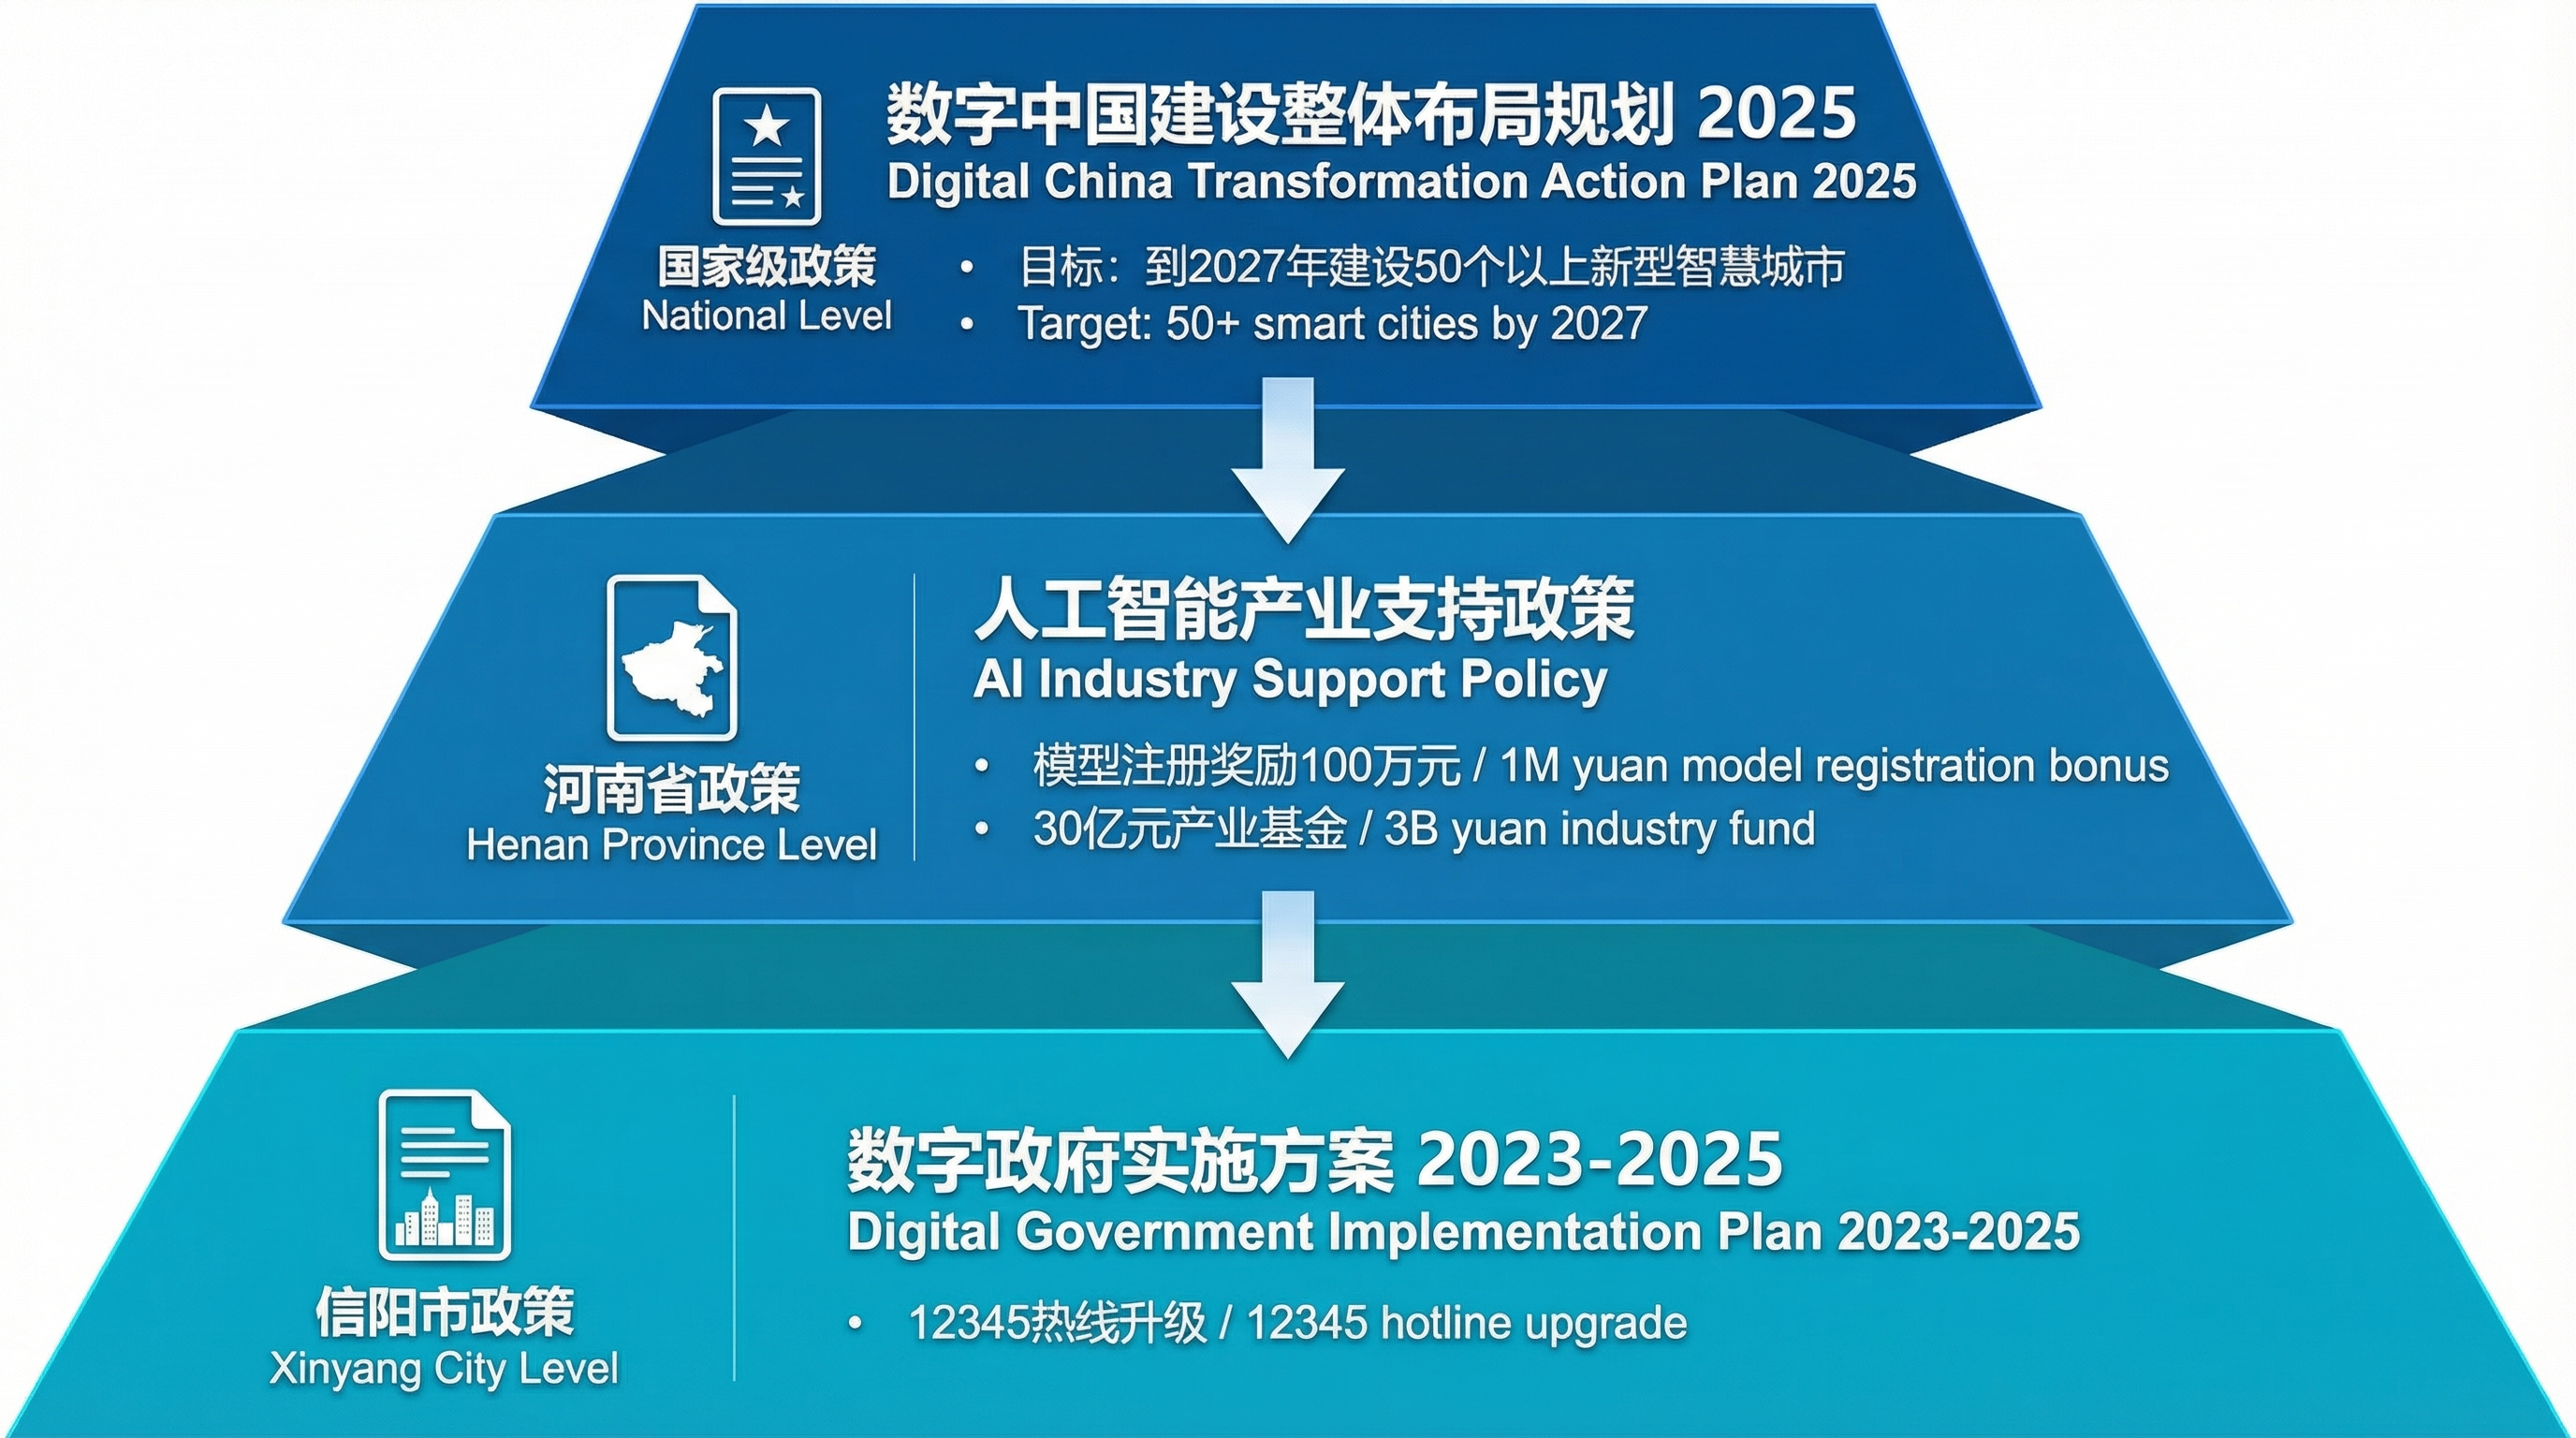
\includegraphics[width=0.85\textwidth]{../picture/fig01_policy_system.png}
\caption{国家-省-市三级政策支持体系图}
\end{figure}

\subsubsection{行业背景}

\textbf{舆情监测市场高速增长}。根据行业调研数据,2024年全球舆情监测系统市场规模约23.15亿美元,预计2031年将达40.50亿美元,年复合增长率8.1\%\textsuperscript{[5]}。中国市场增速领跑全球,2025年预计突破72.4亿元人民币,增速高达26.4\%\textsuperscript{[6]}。

\textbf{行业痛点亟待解决}。当前舆情监测行业存在五大核心痛点:一是\textbf{数据覆盖不全},主流产品聚焦头部平台,对中小网站、短视频、图片等多模态内容的覆盖不足,漏检率高达15-30\%;二是\textbf{智能化程度低},传统系统依赖关键词匹配和人工审核,日均需投入3-5名分析师进行舆情研判,效率低下且成本高昂;三是\textbf{可视化单一},绝大多数产品仍采用传统2D图表和列表展示,难以直观呈现舆情的时空分布与演化态势;四是\textbf{决策支持弱},现有系统侧重于监测和分析环节,缺乏走向预测和决策模拟能力,用户"只知道发生了什么"却"不知道该怎么办";五是\textbf{下沉市场空白},主流产品年费动辄数万至数十万元,地级市、县区及中小企业难以承担,形成显著的市场空白。

\begin{figure}[H]
\centering
\includegraphics[width=0.85\textwidth]{../picture/fig02_market_trend.png}
\caption{中国舆情监测市场规模增长趋势图(2020-2030)}
\end{figure}

\subsubsection{技术背景}

\textbf{大模型技术突破}为智能舆情分析提供了可能。2025年,GPT-5、讯飞星火4.0等主流大模型在情感分析基准测试上的准确率已达94.7\%,远超传统方法的75-85\%\textsuperscript{[8]}。

\textbf{3D可视化技术成熟}。WebGL、Three.js、高德地图JS API 2.0等技术已广泛应用于三维城市可视化场景。

\textbf{AI 3D生成技术兴起}。Tripo AI、TripoSR等工具可在10秒内将文字/图片转换为3D模型。

\subsubsection{地域特色}

\textbf{信阳市}作为河南省地级市,具有独特的区位优势和发展需求,是本项目理想的首批落地场景。信阳地处鄂豫皖三省交界,是著名的革命老区,红色文化资源丰富,舆情场景具有鲜明地域特色。作为中国十大名茶"信阳毛尖"的原产地,茶产业相关的品牌舆情、消费维权、产地保护等议题关注度持续较高。信阳市常住人口超过600万,民生诉求呈现多元化特征,涵盖交通出行、教育医疗、环境保护、消费维权等多个领域。目前信阳市已建成12345市民服务热线平台,初步具备数字政务基础,但智能化分析能力仍有较大提升空间,亟需引入AI技术实现舆情监测的智能化升级。

\subsection{项目优势}

\subsubsection{技术优势}

\begin{table}[H]
\centering
\caption{技术优势总览}
\begin{tabular}{L{3cm}L{10cm}}
\toprule
\textbf{优势维度} & \textbf{具体内容} \\
\midrule
大模型驱动 & 深度集成讯飞星火4.0 Ultra,128K上下文,情感识别准确率超90\% \\
多Agent协作 & 基于LangGraph构建分析-预测-决策-模拟四Agent协作体系 \\
3D可视化 & 高德地图3D + Three.js,支持全国-省-市-县四级穿透 \\
AI场景还原 & Tripo AI生成舆情现场3D模型,实现"看见新闻现场" \\
语音交互 & 讯飞TTS/ASR实现语音播报预警与语音指令控制 \\
轻量化部署 & 云原生架构,支持SaaS订阅,降低使用门槛 \\
\bottomrule
\end{tabular}
\end{table}

\subsubsection{团队优势}

本项目团队具备完成系统开发所需的综合能力。在\textbf{专业构成}方面,团队成员涵盖计算机科学、大数据技术、人工智能等相关专业背景,形成了前端开发、后端架构、AI算法、产品设计等多角色协作的团队结构。在\textbf{技术储备}方面,团队成员具备Web全栈开发、数据可视化、机器学习模型调用等项目实践经历,熟悉Vue3、Python、FastAPI、讯飞星火API等核心技术栈,前端原型已开发完成并验证了技术路线的可行性。在\textbf{本地资源}方面,团队立足信阳学院,对信阳市政务需求和本地舆情特征有切身了解,便于开展需求调研、用户访谈和试点推广,具备"接地气"的产品设计优势。

\subsubsection{差异化优势}

\begin{table}[H]
\centering
\caption{差异化优势对比}
\begin{tabular}{L{2.5cm}L{5cm}L{5.5cm}}
\toprule
\textbf{对比维度} & \textbf{主流产品} & \textbf{智舆系统} \\
\midrule
目标市场 & 省级/大型企业 & 地级市/县域/中小企业 \\
价格定位 & 3-100万元/年 & 万元级/免费增值模式 \\
可视化方式 & 2D图表为主 & 3D地图沉浸式体验 \\
决策支持 & 监测+分析 & 监测+分析+预测+模拟 \\
部署方式 & 私有化为主 & SaaS+轻量化私有化 \\
AI生成能力 & 无 & 舆情场景3D模型生成 \\
\bottomrule
\end{tabular}
\end{table}

% 第二章 项目内容
\section{项目内容}

\subsection{项目界面}

\subsubsection{系统架构}

智舆系统采用\textbf{前后端分离、分层解耦}的现代化架构设计:

\begin{table}[H]
\centering
\caption{系统架构分层}
\begin{tabular}{L{3cm}L{7cm}L{2cm}}
\toprule
\textbf{层级} & \textbf{技术组件} & \textbf{状态} \\
\midrule
前端展示层 & Vue3 + Vite + 高德地图3D + Three.js + ECharts + Element Plus + TailwindCSS + Pinia + Socket.io & 已实现 \\
后端服务层 & FastAPI + Celery + Redis + WebSocket & 开发中 \\
AI分析层 & 讯飞星火4.0 + LangGraph多Agent + LoRA微调 + RAG & 开发中 \\
3D生成层 & Tripo AI / Meshy + 3D Gaussian Splatting + TripoSR & 规划中 \\
语音交互层 & 讯飞TTS + 讯飞ASR + 实时语音流式交互 & 规划中 \\
数据采集层 & MediaCrawler + Scrapy + Playwright + 官方API接口 & 规划中 \\
数据存储层 & PostgreSQL + Elasticsearch + MinIO + Chroma(向量库) & 规划中 \\
\bottomrule
\end{tabular}
\end{table}

\begin{figure}[H]
\centering
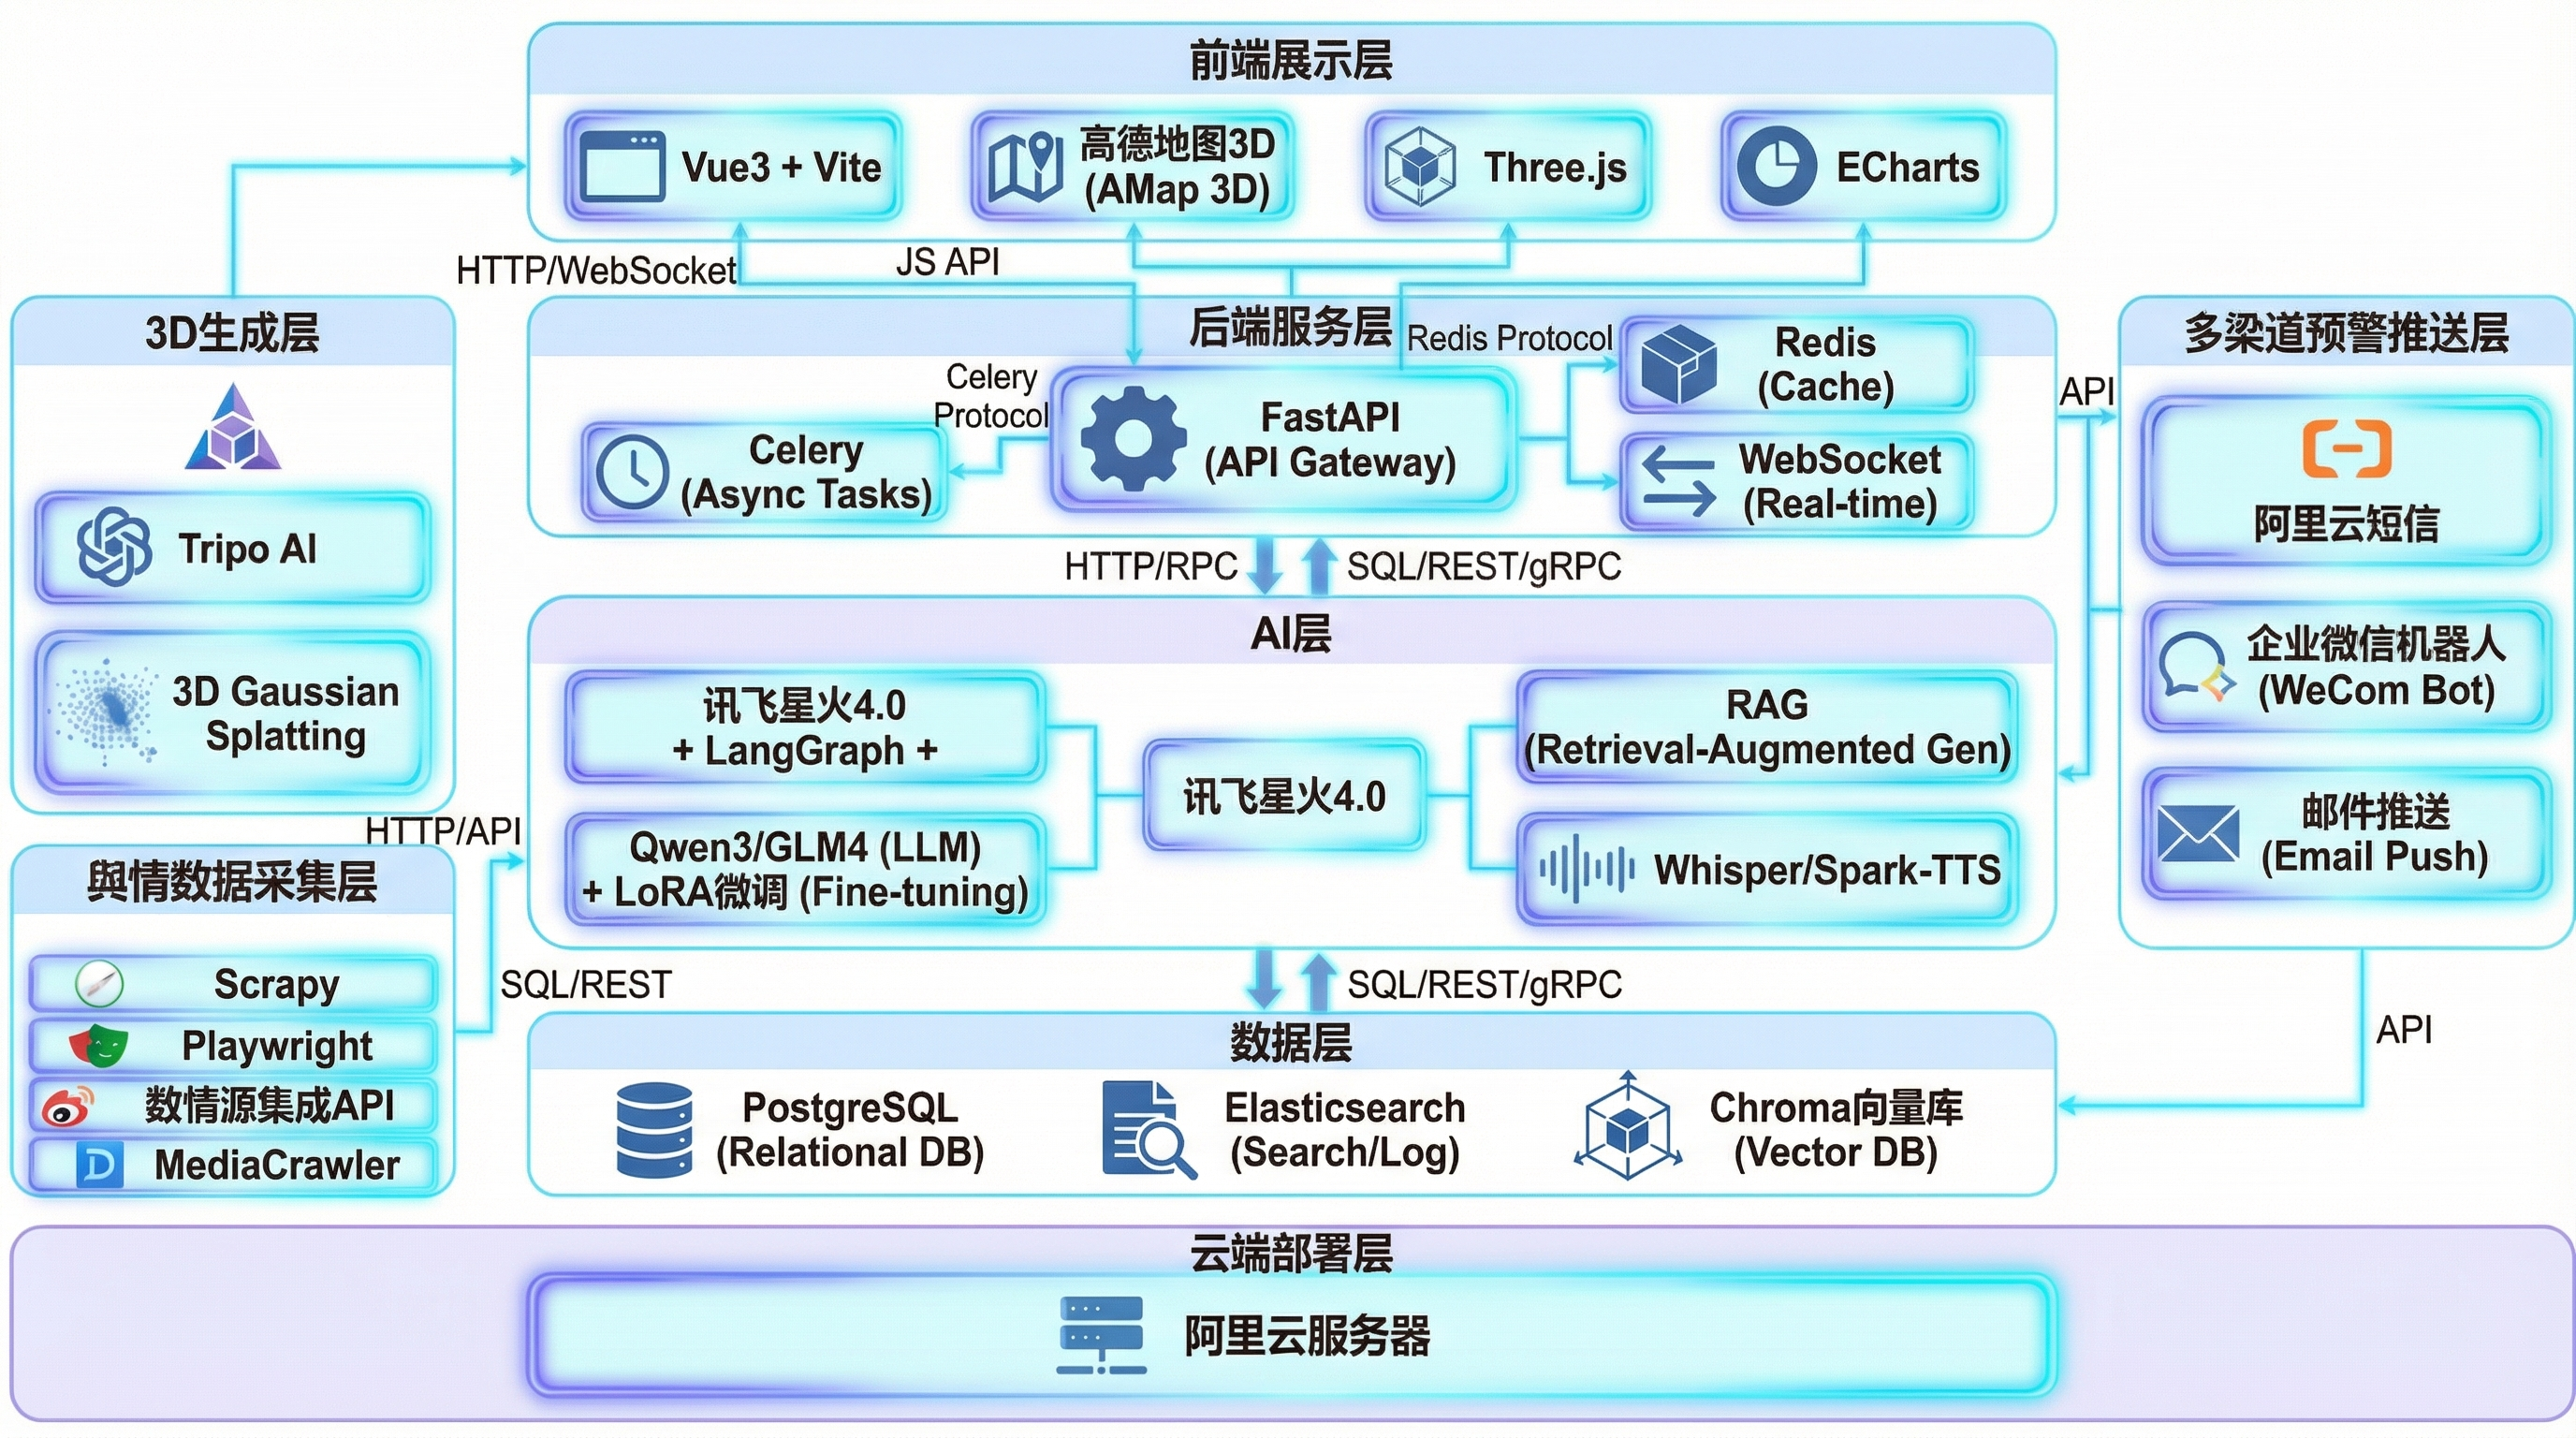
\includegraphics[width=0.85\textwidth]{../picture/fig04_architecture.png}
\caption{系统整体架构图}
\end{figure}

\subsubsection{功能模块}

系统包含\textbf{六大核心功能模块}:

\textbf{模块一:实时舆情监测} -- 多源数据采集,覆盖微博、抖音、小红书等主流平台;多模态解析;实时预警推送。

\begin{figure}[H]
\centering
\includegraphics[width=0.4\textwidth]{../source/UI/筛选界面.png}
\caption{实时舆情监测筛选界面}
\end{figure}

\textbf{模块二:智能舆情分析} -- 情感极性分析(准确率超90\%);主题聚类;传播路径追踪;影响力评估。

\begin{figure}[H]
\centering
\begin{subfigure}[b]{0.48\textwidth}
    \includegraphics[width=\textwidth]{picture/ui_ai_analysis.png}
    \caption{AI智能分析面板}
\end{subfigure}
\hfill
\begin{subfigure}[b]{0.48\textwidth}
    \includegraphics[width=\textwidth]{picture/ui_wordcloud.png}
    \caption{舆情关键词云}
\end{subfigure}
\caption{智能舆情分析模块界面}
\end{figure}

\textbf{模块三:3D地图可视化} -- 四级区域穿透(全国$\rightarrow$省份$\rightarrow$地级市$\rightarrow$县级);3D建筑高亮;热力图叠加;飞行动画。

\textbf{模块四:AI场景还原} -- 文字转3D;图片转3D;地图叠加。

\begin{figure}[H]
\centering
\includegraphics[width=0.85\textwidth]{../source/UI/3D建筑+场景还原.png}
\caption{3D建筑与场景还原界面}
\end{figure}

\textbf{模块五:走向预测与决策模拟} -- 趋势预测;多场景推演;决策建议;效果模拟。

\begin{figure}[H]
\centering
\begin{subfigure}[b]{0.48\textwidth}
    \includegraphics[width=\textwidth]{picture/ui_trend_analysis.png}
    \caption{舆情趋势预测}
\end{subfigure}
\hfill
\begin{subfigure}[b]{0.48\textwidth}
    \includegraphics[width=\textwidth]{picture/ui_decision_sim.png}
    \caption{决策模拟器}
\end{subfigure}
\caption{走向预测与决策模拟模块界面}
\end{figure}

\textbf{模块六:语音交互与播报} -- 语音预警;语音指令;智能问答。

\begin{figure}[H]
\centering
\includegraphics[width=0.75\textwidth]{../picture/fig05_modules.png}
\caption{六大功能模块关系图}
\end{figure}

\subsubsection{界面设计}

系统界面采用\textbf{赛博朋克+玻璃拟态(Glassmorphism)}设计风格:

\textbf{主界面布局}采用五区域设计。顶部\textbf{Dynamic Island导航栏}集成时间显示、功能图标快捷入口、智能搜索与系统设置,提供一站式操作入口。左侧\textbf{舆情监控筛选栏}支持按风险等级(高/中/低)、分类标签(交通/民生/消费/餐饮/环境)、时间范围(24小时/3天/7天/30天)进行多维度过滤,并实时展示舆情列表。中央\textbf{3D地图主视图}基于高德地图JS API 2.0实现三维城市可视化,支持区域边界霓虹渲染、舆情热点标注、关键词浮动展示等效果。右侧\textbf{智能分析面板}展示AI生成的情感分析结果、趋势预测曲线、舆情词云、决策模拟交互与结果展示。右下角\textbf{图层控制工具栏}提供热力图、边界线、3D建筑模型、悬浮标志、事件关联线等可视化图层的开关控制。

\textbf{视觉特色}:霓虹色彩(Cyan-400主色调)、毛玻璃半透明效果、动态光效与粒子、3D纵深空间感。

\textbf{响应式设计}:系统采用单一代码库,通过CSS媒体查询适配不同屏幕。Web/PC端(lg/xl)呈现完整三栏布局(侧边栏+核心地图+右侧面板),支持鼠标精细操作和复杂3D交互;移动端(xs/sm)采用单列布局,地图作为背景,侧边栏收起为汉堡菜单,功能面板转为底部抽屉(Bottom Sheet),触控区域经过优化以适配手指操作。

\textbf{用户交互流程}:系统引导用户完成从"发现问题"到"解决问题"的完整闭环,分为四个阶段。\textbf{感知阶段}:3D地图上某区域出现红色脉冲警报,左侧实时列表弹出"突发"标签的新闻条目,用户点击地图红点或列表条目触发下一阶段。\textbf{分析阶段}:地图视角自动平滑推拉至事发地点,右侧面板滑出事件详情卡片,展示AI生成的事件摘要、情绪占比分析,若可用则弹出3D现场还原全息影像。\textbf{预测阶段}:地图上显示动态箭头预示舆情可能扩散区域,趋势图展示未来24小时热度预测曲线,AI助手弹出决策建议。\textbf{模拟阶段}:用户打开决策模拟器,选择或输入决策方案,系统即时计算后地图警报区域根据模拟结果变化,趋势图生成虚线分支对比不同决策下的未来走向。

\begin{figure}[H]
\centering
\includegraphics[width=0.95\textwidth]{../source/UI/ui_main_interface.png}
\caption{系统主界面}
\end{figure}

\begin{figure}[H]
\centering
\makebox[\textwidth][c]{\includegraphics[width=1.3\textwidth]{../source/UI/ui_elements_guide.png}}
\caption{界面元素详解图}
\end{figure}

\begin{figure}[H]
\centering
\includegraphics[width=0.9\textwidth]{../picture/fig07_interaction_flow.png}
\caption{界面交互流程图}
\end{figure}

\subsection{项目特色}

\subsubsection{核心创新点}

\textbf{创新点一:AI驱动的舆情场景3D还原}

这是本项目最具创新性的功能。智舆系统创新性地引入\textbf{AI 3D生成技术},可根据舆情内容自动生成现场3D模型。

\textbf{技术实施路径}:首先,系统通过讯飞星火4.0大模型对舆情内容进行语义理解,提取关键场景元素(如"建筑物"、"车辆"、"人群"等),并根据事件类型生成结构化场景描述JSON。对于\textbf{文字舆情},系统将场景描述转换为Tripo AI可识别的Prompt,调用text-to-3D API生成模型,平均耗时约10秒。对于\textbf{图片舆情},采用TripoSR开源模型进行单图3D重建,该模型基于Transformer架构,支持本地部署,推理速度约500ms/张。对于\textbf{视频舆情},首先通过讯飞LFASR进行音频转写,提取视频关键帧进行3D重建,并将转写文本与3D场景融合,生成完整的可交互场景。生成的3D模型统一转换为GLTF格式,通过Three.js加载并叠加到高德地图GLCustomLayer上,实现\textbf{"在地图上看见新闻现场"}的沉浸式体验。

\begin{figure}[H]
\centering
\includegraphics[width=0.9\textwidth]{../picture/fig08_ai_3d_workflow.png}
\caption{AI 3D场景还原技术流程图}
\end{figure}

\textbf{创新点二:多Agent协作的决策模拟系统}

基于\textbf{LangGraph}框架构建多Agent协作体系:

\begin{table}[H]
\centering
\caption{多Agent协作体系}
\begin{tabular}{L{2.5cm}L{3cm}L{3.5cm}L{4cm}}
\toprule
\textbf{Agent} & \textbf{职责} & \textbf{输入} & \textbf{输出} \\
\midrule
分析Agent & 舆情深度分析 & 原始舆情数据 & 情感、主题、影响力分析 \\
预测Agent & 走向趋势预测 & 分析结果+历史数据 & 乐观/中性/悲观场景 \\
决策Agent & 生成应对方案 & 预测结果 & 多套决策建议 \\
模拟Agent & 模拟执行效果 & 用户选择的决策 & 效果评估报告 \\
\bottomrule
\end{tabular}
\end{table}

\textbf{技术实施路径}:LangGraph采用有向图结构管理Agent状态流转,系统状态定义为$S = \{s_{\text{input}}, s_{\text{analysis}}, s_{\text{prediction}}, s_{\text{decision}}, s_{\text{simulation}}\}$,状态转移函数为:
\begin{equation}
s_{t+1} = f_{\text{agent}}(s_t, \text{LLM}(s_t))
\end{equation}
其中$f_{\text{agent}}$为当前激活Agent的处理函数,$\text{LLM}(s_t)$为讯飞星火4.0基于当前状态生成的推理结果。系统通过\texttt{StateGraph}定义节点(Node)和边(Edge),每个Agent作为独立节点,边定义条件路由逻辑。分析Agent输出情感得分$e \in [-1, 1]$和影响力指数$I$,当$e < -0.5$且$I > 0.7$时触发预警分支;预测Agent基于历史数据拟合趋势曲线$\hat{y}(t) = \alpha \cdot y(t-1) + \beta \cdot \Delta y + \epsilon$,生成未来24/48/72小时热度预测;决策Agent根据预测场景生成3-5套应对方案并评估风险收益比;模拟Agent接收用户选择的方案,通过蒙特卡洛模拟生成$N=1000$条演化路径,输出置信区间和效果评估报告。

\begin{figure}[H]
\centering
\includegraphics[width=0.8\textwidth]{../picture/fig09_multi_agent.png}
\caption{多Agent决策模拟架构图}
\end{figure}

\textbf{创新点三:四级区域穿透的3D地图可视化}

突破传统舆情系统的2D展示局限,实现\textbf{全国$\rightarrow$省份$\rightarrow$地级市$\rightarrow$县级}的四级3D可视化穿透:

系统基于高德地图JS API 2.0的Map3D模式构建三维地图底图,通过\texttt{AMap.DistrictSearch}API获取行政区划边界数据。在全国视图(Zoom 4-6)层级,采用降采样算法对边界点进行简化,保留大面积区域的Top 50多边形,以霓虹双层线条渲染国境轮廓,展示全国舆情热度分布。在省份视图(Zoom 6-8)层级,加载省级边界并渲染地市分割,以颜色深浅表征各地市舆情活跃度。在地市视图(Zoom 8-12)层级,加载城区边界并开启3D建筑图层,对舆情事件关联建筑进行霓虹高亮标注。在县区视图(Zoom 12+)层级,加载街道级详细地图,展示舆情事件的精确坐标与关联建筑。视图切换采用"高空跳跃"动画,当目标距离超过5度(~550km)时,先缩放至全国视角再飞入目标区域,提供流畅的空间感知体验。

\begin{figure}[H]
\centering
\begin{minipage}[b]{0.48\textwidth}
\centering
\includegraphics[width=\textwidth]{../source/UI/ui_drill_1_national.png}
\subcaption{全国视图}
\end{minipage}
\hfill
\begin{minipage}[b]{0.48\textwidth}
\centering
\includegraphics[width=\textwidth]{../source/UI/ui_drill_2_province.png}
\subcaption{省级视图}
\end{minipage}
\vspace{0.5em}
\begin{minipage}[b]{0.48\textwidth}
\centering
\includegraphics[width=\textwidth]{../source/UI/ui_drill_3_city.png}
\subcaption{市级视图}
\end{minipage}
\hfill
\begin{minipage}[b]{0.48\textwidth}
\centering
\includegraphics[width=\textwidth]{../source/UI/ui_drill_4_district.png}
\subcaption{区级视图}
\end{minipage}
\caption{四级区域穿透示意图}
\end{figure}

\textbf{创新点四:讯飞技术深度集成}

\begin{table}[H]
\centering
\caption{讯飞技术应用}
\begin{tabular}{L{3cm}L{4.5cm}L{5.5cm}}
\toprule
\textbf{讯飞技术} & \textbf{应用场景} & \textbf{技术价值} \\
\midrule
星火4.0 Ultra & 舆情分析、趋势预测、决策生成 & 128K上下文,中文理解能力领先 \\
星火Lite & 日常对话、轻量任务 & 永久免费,降低运营成本 \\
在线TTS & 语音预警播报 & 超拟人语音,多音色选择 \\
实时ASR & 语音指令输入 & 实时转写,语音操控地图 \\
LFASR & 视频舆情音频转写 & 长音频转写,提取视频内容 \\
NLP & 情感分析、关键词提取 & 细粒度中文语义理解 \\
\bottomrule
\end{tabular}
\end{table}

\textbf{技术实施路径}:讯飞技术通过统一的API网关进行集成,采用异步调用模式提升响应效率。\textbf{星火大模型}通过REST API调用,请求体包含\texttt{messages}对话历史和\texttt{functions}工具定义,响应采用流式SSE(Server-Sent Events)返回,支持实时展示生成过程。\textbf{语音合成TTS}采用WebSocket长连接,将文本分片传输,服务端实时返回PCM音频流,前端通过Web Audio API播放,延迟控制在200ms以内。\textbf{语音识别ASR}同样采用WebSocket,前端通过\texttt{MediaRecorder}采集麦克风音频,以16kHz采样率、16bit位深编码后实时上传,服务端返回中间识别结果和最终结果,支持"语音操控地图"等指令识别。\textbf{长音频转写LFASR}采用HTTP异步模式,先上传音频文件获取\texttt{task\_id},轮询查询转写进度,完成后获取带时间戳的文本结果。所有API调用均封装为Python/JavaScript SDK,通过环境变量管理\texttt{APPID}、\texttt{APIKey}、\texttt{APISecret}等鉴权信息。

\textbf{创新点五:城市模型矩阵}

针对不同城市/省份的舆情特征差异,系统采用\textbf{LoRA微调技术}为每个区域训练专属的轻量级适配器,形成"城市模型矩阵":

\begin{table}[H]
\centering
\caption{城市模型矩阵架构}
\begin{tabular}{L{2.5cm}L{4cm}L{6.5cm}}
\toprule
\textbf{层级} & \textbf{模型配置} & \textbf{作用} \\
\midrule
基座模型 & 讯飞星火4.0 Ultra & 提供通用舆情理解与推理能力 \\
省级适配器 & LoRA-河南/LoRA-广东/... & 学习省级方言、地域文化、本地热点 \\
市级适配器 & LoRA-信阳/LoRA-郑州/... & 精细化本地舆情分析,识别区县特征 \\
\bottomrule
\end{tabular}
\end{table}

\textbf{技术实施路径}:LoRA(Low-Rank Adaptation)技术的核心思想是在预训练模型的注意力层中插入低秩分解矩阵。对于权重矩阵$W_0 \in \mathbb{R}^{d \times k}$,LoRA将其更新分解为:
\begin{equation}
W = W_0 + \Delta W = W_0 + BA
\end{equation}
其中$B \in \mathbb{R}^{d \times r}$,$A \in \mathbb{R}^{r \times k}$,$r \ll \min(d,k)$为秩参数,通常取$r=8$即可达到良好效果。通过仅训练$B$和$A$矩阵,可训练参数量从数十亿降至数百万(0.1\%),消费级GPU(16GB显存)即可完成城市级舆情适配器训练。系统支持\textbf{动态加载},根据用户查看区域自动切换对应LoRA适配器,新增城市只需训练新适配器,无需重训基座模型,实现\textbf{增量扩展}。

\subsubsection{技术亮点}

\textbf{亮点一:前端已实现完整功能原型}

本项目前端已采用\textbf{Vue3 + Vite + 高德地图3D + Three.js + ECharts}技术栈实现完整功能原型,包括赛博朋克风格UI、3D地图可视化与四级穿透、城市自动检测、热力图与边界渲染、飞行动画等。

\begin{figure}[H]
\centering
\begin{minipage}[b]{0.48\textwidth}
\centering
\includegraphics[width=\textwidth]{../source/UI/ui_ai_analysis.png}
\subcaption{AI智能分析}
\end{minipage}
\hfill
\begin{minipage}[b]{0.48\textwidth}
\centering
\includegraphics[width=\textwidth]{../source/UI/ui_decision_sim.png}
\subcaption{决策模拟}
\end{minipage}
\vspace{0.5em}
\begin{minipage}[b]{0.48\textwidth}
\centering
\includegraphics[width=\textwidth]{../source/UI/ui_trend_analysis.png}
\subcaption{趋势分析}
\end{minipage}
\hfill
\begin{minipage}[b]{0.48\textwidth}
\centering
\includegraphics[width=\textwidth]{../source/UI/ui_wordcloud.png}
\subcaption{关键词云}
\end{minipage}
\caption{已实现功能截图集}
\end{figure}

\textbf{亮点二:模块化可扩展架构}

系统采用\textbf{微服务架构思想},各功能模块松耦合、可独立部署。

\textbf{技术实施路径}:系统按功能边界划分为6个独立服务模块,通过RESTful API和WebSocket进行通信。前端采用Vue3组件化开发,按功能域划分\texttt{features/}目录(Map、Monitor、Analysis、Simulation、Voice),共享组件置于\texttt{ui/}目录,状态管理通过Pinia实现跨组件数据共享。后端采用FastAPI构建,每个业务模块对应独立的Router,通过依赖注入(Dependency Injection)解耦服务层与数据层。模块间通信遵循事件驱动模式,舆情更新通过Redis Pub/Sub广播至各订阅模块,前端通过Socket.io接收实时推送。新增功能只需添加对应模块并注册路由,无需修改核心代码,实现\textbf{开闭原则}(对扩展开放、对修改关闭)。

\textbf{亮点三:多源数据采集能力}

基于\textbf{MediaCrawler}开源框架,实现7大主流平台(小红书、抖音、微博、B站、快手、知乎、贴吧)一站式数据采集。

\textbf{技术实施路径}:数据采集采用三层架构设计。\textbf{采集层}基于MediaCrawler + Playwright实现,通过模拟真实浏览器行为绕过反爬机制,支持Cookie登录和二维码登录两种认证方式,登录态自动缓存避免重复认证。\textbf{调度层}基于Celery + Redis构建分布式任务队列,支持定时采集(Cron表达式配置)和实时触发(热点事件监控),通过IP代理池轮换防止封禁。\textbf{清洗层}对原始数据进行结构化处理,提取核心字段(标题、正文、发布时间、互动数据、地理位置等),调用讯飞NLP进行情感标注和关键词提取,最终存入PostgreSQL(结构化数据)和Elasticsearch(全文检索)。数据流转遵循ETL范式:
\begin{equation}
D_{\text{raw}} \xrightarrow{\text{Extract}} D_{\text{struct}} \xrightarrow{\text{Transform}} D_{\text{enriched}} \xrightarrow{\text{Load}} \text{DB}
\end{equation}
其中$D_{\text{enriched}}$包含原始内容、情感得分$e$、关键词集合$K$、地理坐标$(lat, lng)$等增强字段。

\subsubsection{与同类产品的差异}

\begin{table}[H]
\centering
\caption{与同类产品对比}
\small
\begin{tabular}{L{2cm}L{2.3cm}L{2.3cm}L{2.3cm}L{3cm}}
\toprule
\textbf{维度} & \textbf{新浪舆情通} & \textbf{人民网舆情} & \textbf{清博大数据} & \textbf{智舆系统} \\
\midrule
定位客群 & 大型政企 & 政府机构 & 高校/媒体 & 地级市/中小企业 \\
年费价格 & 3-25万 & 5-50万 & 2-20万 & 万元级 \\
3D可视化 & 无 & 无 & 无 & 四级穿透3D地图 \\
AI场景还原 & 无 & 无 & 无 & 舆情3D模型生成 \\
决策模拟 & 无 & 无 & 无 & 多Agent决策推演 \\
语音交互 & 无 & 无 & 无 & 讯飞TTS/ASR \\
\bottomrule
\end{tabular}
\end{table}

% 第三章 项目可行性
\section{项目可行性}

\subsection{技术可行性}

\subsubsection{核心技术说明}

\textbf{大语言模型技术}

讯飞星火4.0 Ultra作为本项目核心AI引擎,具备完整的舆情分析能力体系。该模型支持128K tokens超长上下文,可处理长篇舆情分析报告与多轮对话,针对中文语境进行深度优化,对网络用语、地方方言、缩略语等特殊表达具有较强的理解能力。讯飞星火API提供成熟稳定的REST API和WebSocket接口,支持情感分析、主题提取、摘要生成、对话问答等多种任务类型。此外,系统还集成\textbf{讯飞NLP}能力,用于细粒度情感分析和关键词提取,进一步提升舆情内容理解的准确性。

\textbf{情感分析算法}:系统采用基于Transformer的序列分类模型进行情感极性判断。对于输入文本$X = \{x_1, x_2, ..., x_n\}$,经过讯飞星火编码器得到隐藏表示$H = \text{Encoder}(X)$,通过分类头输出情感概率分布:
\begin{equation}
P(y|X) = \text{Softmax}(W_c \cdot H_{[CLS]} + b_c)
\end{equation}
其中$H_{[CLS]}$为[CLS]位置的隐藏向量,$y \in \{+1, 0, -1\}$(分别表示正面、中性、负面)。根据行业评测,2025年主流系统情感识别准确率普遍超过90\%,对网络用语的情感极性判断准确率超92\%\textsuperscript{[7]}。

\textbf{3D可视化技术}:系统基于高德地图JS API 2.0构建3D可视化底座,该API原生支持3D地图视图、建筑层渲染、区域边界查询等功能。Three.js作为成熟的WebGL封装框架,通过\texttt{GLCustomLayer}与高德地图无缝对接,用于渲染自定义3D模型、粒子效果、流动线等高级可视化元素。WebGL为浏览器原生支持技术,无需安装插件,兼容性覆盖98\%以上的现代浏览器。

\textbf{AI 3D生成技术}:系统集成多种前沿AI 3D生成技术。Tripo AI支持文字/图片/草图到3D模型的快速生成,平均生成时间约10秒,通过REST API调用。TripoSR是Stability AI开源的单图3D重建模型,基于Transformer架构,支持本地部署,推理速度约500ms。该模型将单张图像$I \in \mathbb{R}^{H \times W \times 3}$编码为特征向量,通过解码器生成三维点云$P = \{(x_i, y_i, z_i)\}_{i=1}^N$,经过网格重建输出GLTF格式模型。3D Gaussian Splatting是新兴的实时场景重建技术,通过一组高斯分布$G = \{(\mu_i, \Sigma_i, c_i, \alpha_i)\}$表示场景,支持实时渲染与视角切换。

\textbf{小模型微调技术}:为实现城市模型矩阵的低成本训练,系统采用多种参数高效微调技术。LoRA(Low-Rank Adaptation)通过低秩分解将微调参数量降低至原模型的0.1\%,16GB显存的消费级GPU即可完成训练。P-Tuning通过在输入层添加可学习的连续提示向量$P = \{p_1, p_2, ..., p_m\}$来引导模型行为,适合多任务共享场景。QLoRA结合4-bit NF4量化与LoRA技术,将基座模型内存占用压缩至原来的1/4,进一步降低部署门槛,使得12GB显存的显卡也能完成微调训练。

\subsubsection{技术路线图}

\begin{table}[H]
\centering
\caption{技术路线规划}
\begin{tabular}{L{2cm}L{2cm}L{8cm}}
\toprule
\textbf{阶段} & \textbf{状态} & \textbf{主要内容} \\
\midrule
Phase 1 & 已完成 & 前端原型:Vue3 + Vite框架搭建、高德地图3D集成、赛博朋克UI设计 \\
Phase 2 & 进行中 & 后端服务:FastAPI框架、讯飞星火API接入、WebSocket实时推送 \\
Phase 3 & 规划中 & AI增强:LangGraph多Agent、走向预测、决策模拟、讯飞TTS/ASR \\
Phase 4 & 规划中 & 3D生成:Tripo AI集成、舆情场景生成、模型地图叠加 \\
Phase 5 & 规划中 & 数据采集:MediaCrawler部署、多平台数据接入、合规风控 \\
\bottomrule
\end{tabular}
\end{table}

\begin{figure}[H]
\centering
\includegraphics[width=0.9\textwidth]{../picture/fig12_gantt.png}
\caption{技术路线甘特图}
\end{figure}

\subsubsection{讯飞技术应用方案}

\begin{table}[H]
\centering
\caption{讯飞技术应用方案}
\begin{tabular}{L{3cm}L{2.5cm}L{4cm}L{3cm}}
\toprule
\textbf{讯飞技术} & \textbf{集成方式} & \textbf{应用场景} & \textbf{预计调用量} \\
\midrule
星火4.0 Ultra & REST API & 舆情分析、决策生成 & 1000次/天 \\
星火Lite & REST API & 日常对话、轻量任务 & 5000次/天 \\
在线TTS & WebSocket & 语音预警播报 & 500次/天 \\
实时ASR & WebSocket & 语音指令输入 & 200次/天 \\
LFASR & HTTP & 视频音频转写 & 50次/天 \\
\bottomrule
\end{tabular}
\end{table}

\subsubsection{开发进度计划}

\begin{table}[H]
\centering
\caption{开发进度计划}
\begin{tabular}{L{2cm}L{1.5cm}L{5cm}L{4cm}}
\toprule
\textbf{阶段} & \textbf{时间} & \textbf{主要任务} & \textbf{交付物} \\
\midrule
需求分析 & 第1周 & 需求调研、技术选型 & 需求文档、技术方案 \\
前端开发 & 第2-3周 & UI实现、地图集成 & 前端原型(已完成) \\
后端开发 & 第4-5周 & API开发、数据库设计 & 后端服务 \\
AI集成 & 第6-7周 & 讯飞API接入、Agent开发 & AI分析功能 \\
功能完善 & 第8周 & 联调测试、Bug修复 & 完整系统 \\
优化上线 & 第9周 & 性能优化、文档编写 & 可演示产品 \\
\bottomrule
\end{tabular}
\end{table}

\subsection{经济可行性}

\subsubsection{成本分析}

\textbf{开发成本}

\begin{table}[H]
\centering
\caption{开发成本}
\begin{tabular}{L{4cm}L{3cm}L{6cm}}
\toprule
\textbf{成本项} & \textbf{金额} & \textbf{说明} \\
\midrule
人力成本 & 0元 & 团队成员学习型投入 \\
硬件成本 & 0元 & 使用现有个人电脑 \\
软件成本 & 0元 & 采用开源技术栈 \\
\textbf{合计} & \textbf{0元} & 无额外开发投入 \\
\bottomrule
\end{tabular}
\end{table}

\textbf{运营成本(月)}

\begin{table}[H]
\centering
\caption{月运营成本}
\begin{tabular}{L{4cm}L{3cm}L{6cm}}
\toprule
\textbf{成本项} & \textbf{金额} & \textbf{说明} \\
\midrule
云服务器 & 50-200元 & 阿里云/腾讯云学生机 \\
讯飞星火API & 0-50元 & Lite免费,Pro按量计费 \\
讯飞TTS/ASR & 0元 & 免费额度 \\
高德地图API & 0元 & 个人开发者免费 \\
Tripo AI & 0-30元 & 免费额度 \\
域名 & 约2.5元 & 30元/年 \\
\textbf{合计} & \textbf{约80-300元/月} & 低成本运营 \\
\bottomrule
\end{tabular}
\end{table}

\subsubsection{收益预测}

\textbf{商业模式设计}:系统采用多元化营收模式。核心收入来自\textbf{SaaS订阅服务},提供基础版(免费)、专业版(2000元/年)、企业版(10000元/年)三个梯度,差异化功能包括数据源数量、分析深度、导出格式、API调用量等。增值收入包括\textbf{定制开发},为政府/企业客户提供个性化功能开发、私有化部署等服务;\textbf{数据报告服务},提供周/月/年度舆情分析报告;\textbf{API能力开放},允许第三方应用调用情感分析、趋势预测等能力。

\textbf{市场规模预估}:以信阳市为例进行潜在客户分析。市级政府部门(宣传部、网信办、应急管理局等)约10个潜在客户,县区政府(8县2区)约10个潜在客户,本地企业(茶企、旅游、地产等)约50家有舆情监测需求。合计约70个潜在客户,假设首年渗透率10\%、平均客单价1万元,首年收入潜力约7万元。随着口碑积累和区域扩展,第二年预计渗透率可提升至20\%,年收入达14万元以上。

\subsubsection{投入产出比}

\begin{table}[H]
\centering
\caption{投入产出分析}
\begin{tabular}{L{5cm}L{8cm}}
\toprule
\textbf{指标} & \textbf{数值} \\
\midrule
首年投入(开发+运营) & 约3000元 \\
首年收入预期 & 约1-7万元 \\
投入产出比 & 3-23倍 \\
盈亏平衡点 & 约4个付费客户 \\
\bottomrule
\end{tabular}
\end{table}

\begin{figure}[H]
\centering
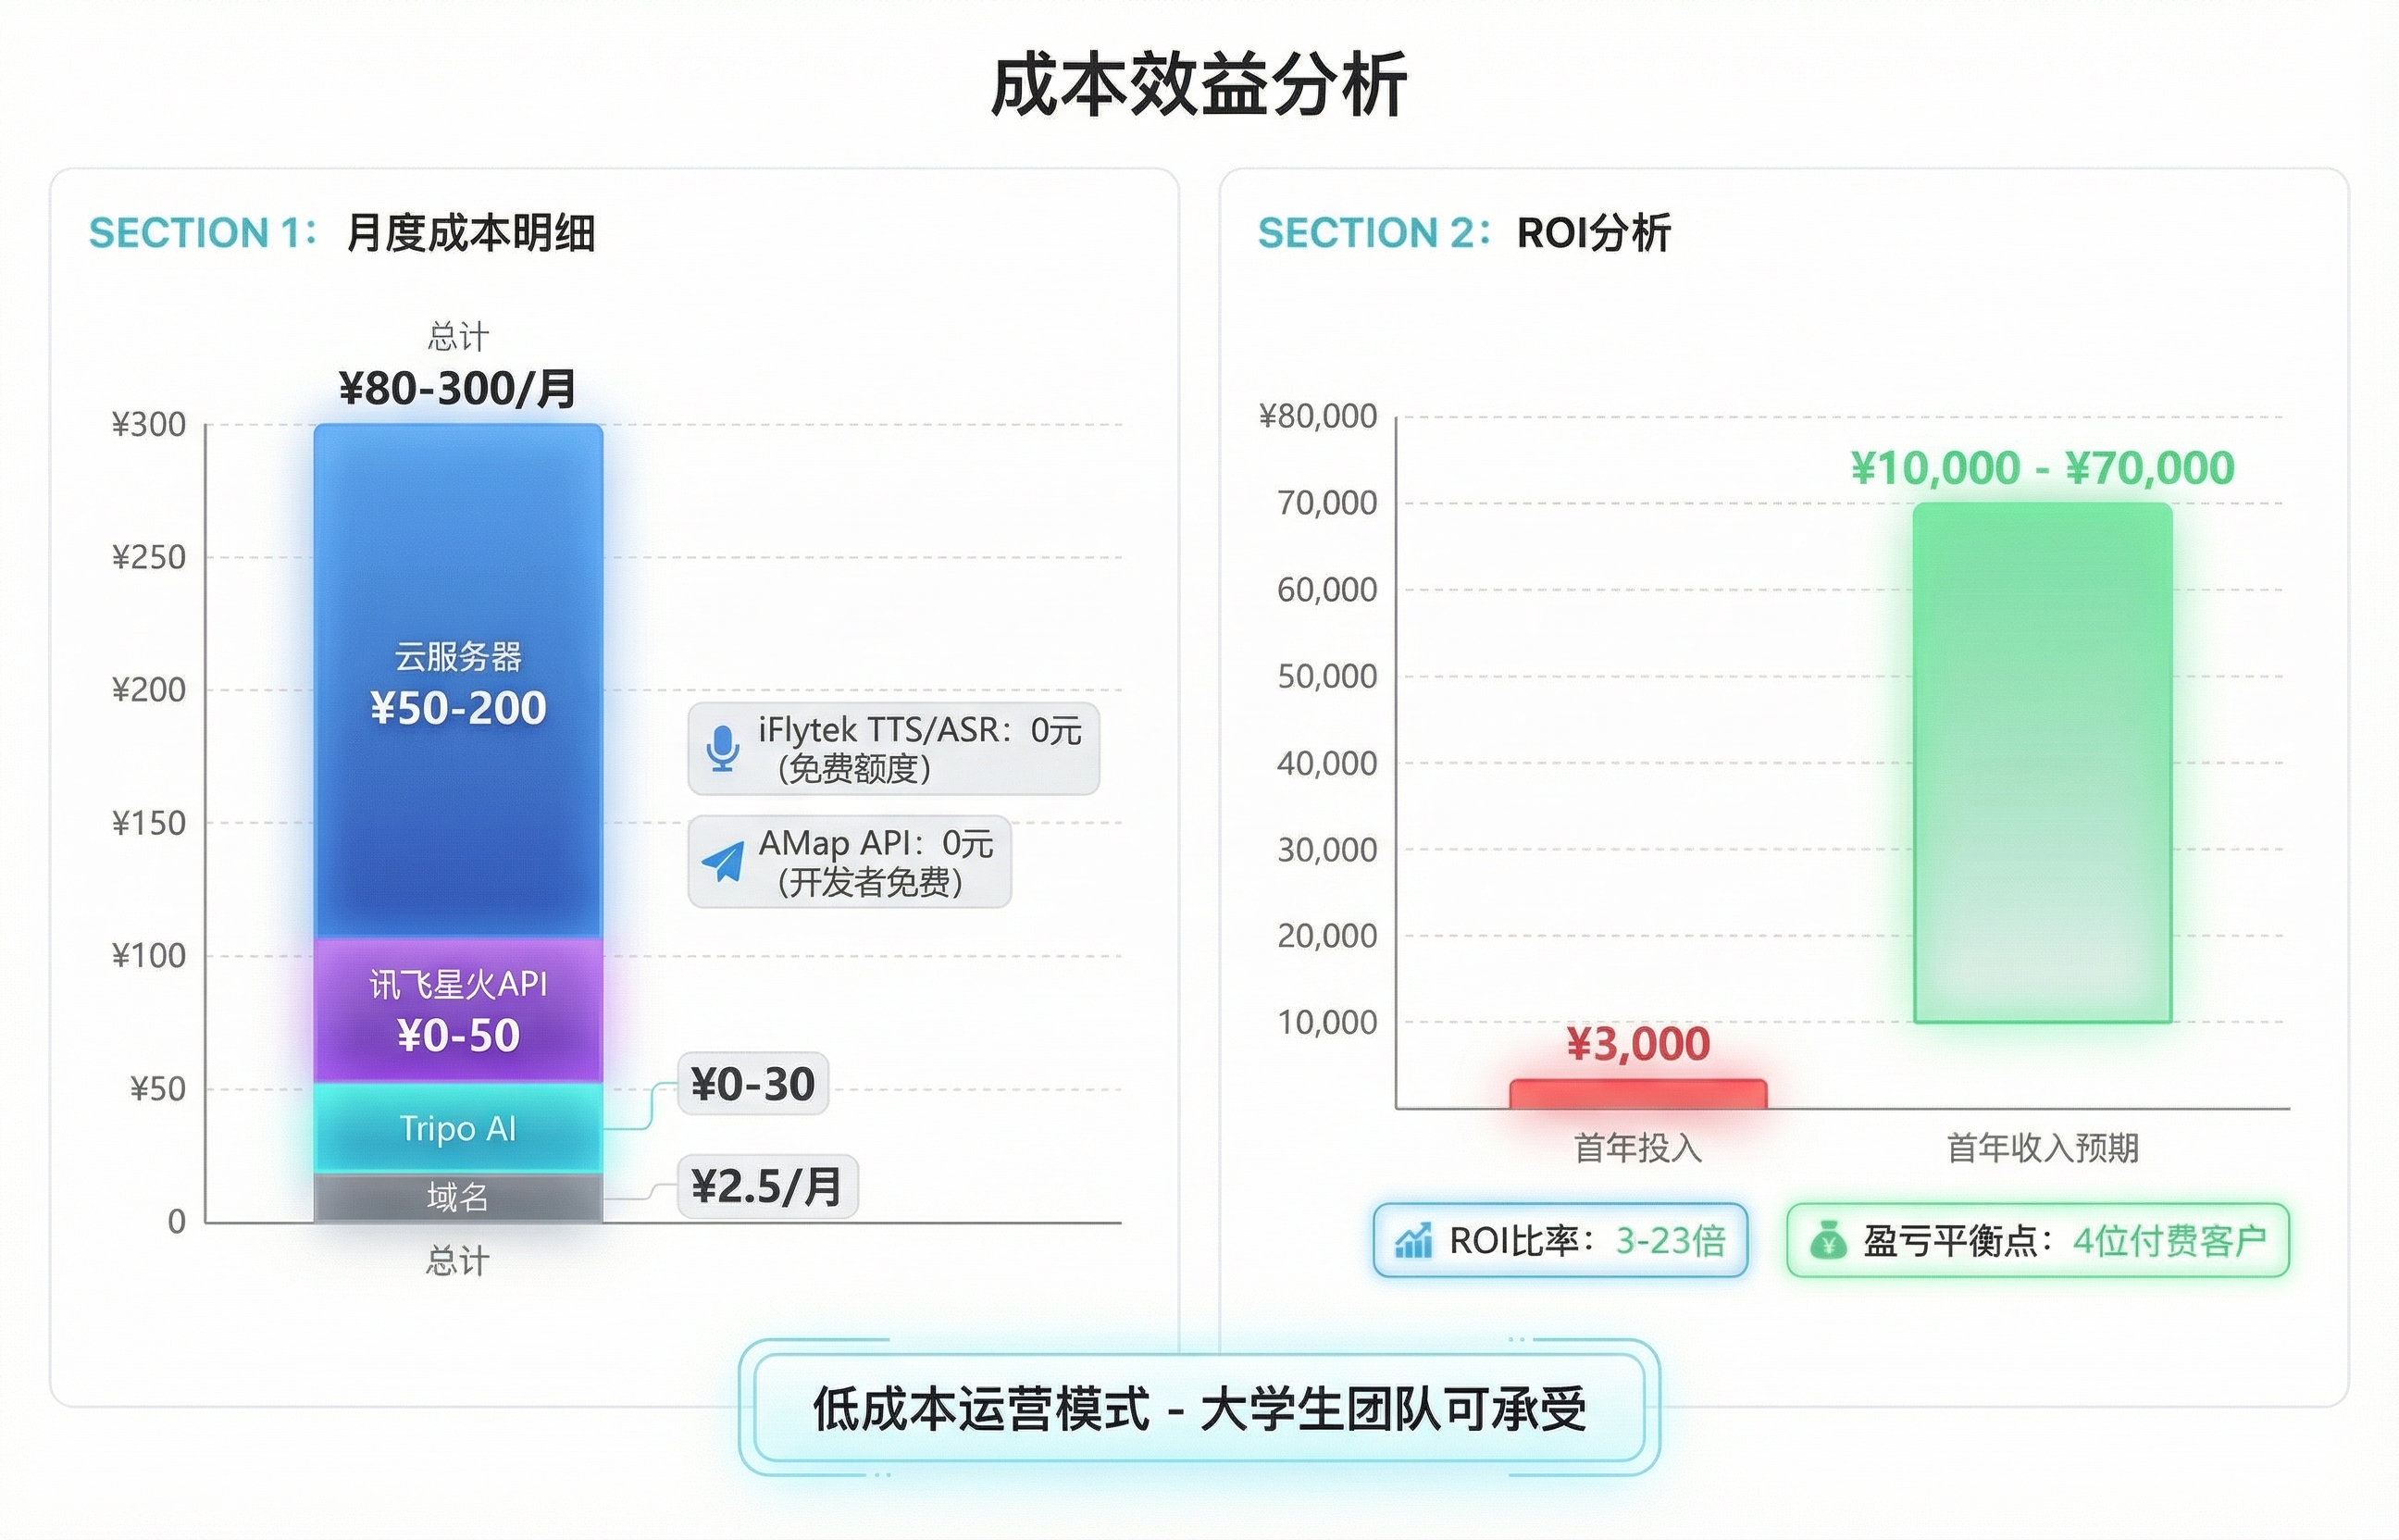
\includegraphics[width=0.85\textwidth]{../picture/fig13_cost_benefit.png}
\caption{成本收益分析图}
\end{figure}

% 第四章 项目市场分析
\section{项目市场分析}

\subsection{市场环境分析}

\subsubsection{PEST分析}

\textbf{Political(政治环境)}:国家层面高度重视数字政府和智慧城市建设,《深化智慧城市发展推进全域数字化转型行动计划》明确提出到 2027年底建成50个以上全域数字化转型城市的目标。河南省设立30亿元人工智能产业基金,对通过国家生成式AI模型备案的企业给予100万元资金支持。舆情管理已纳入城市治理体系,各级政府对舆情监测能力建设需求明确。

\textbf{Economic(经济环境)}:中国舆情监测市场2025年预计突破72.4亿元,年增速高达26.4\%\textsuperscript{[6]},远超全球平均水平。地级市、县域市场存在大量空白,主流产品年费动辄3-100万元,中小客户难以承担,形成显著的价格缝隙市场。AI技术的成熟大幅降低了舆情分析成本,云服务的普及使得轻量化SaaS部署成为可能,中小企业的舆情监测需求正在加速释放。

\textbf{Social(社会环境)}:社交媒体用户规模持续增长,我国网民规模已超过10亿,舆情传播速度显著加快。短视频、直播已成为舆情爆发的主渠道,传统的文字监测手段难以全面覆盖。公众对政府信息透明度和响应速度要求不断提高,企业品牌声誉意识增强,危机公关和品牌维护需求持续上升。

\textbf{Technological(技术环境)}:大语言模型技术已趋成熟,2025年主流系统情感识别准确率普遍超过90\%\textsuperscript{[7]}。多模态分析能力大幅提升,支持图片、视频、音频等多种内容形式的解析。3D可视化技术已广泛普及,WebGL兼容性覆盖98\%以上现代浏览器。AI 3D生成技术快速兴起,秒级模型生成已成为现实,为舆情场景还原提供了技术基础。

\begin{figure}[H]
\centering
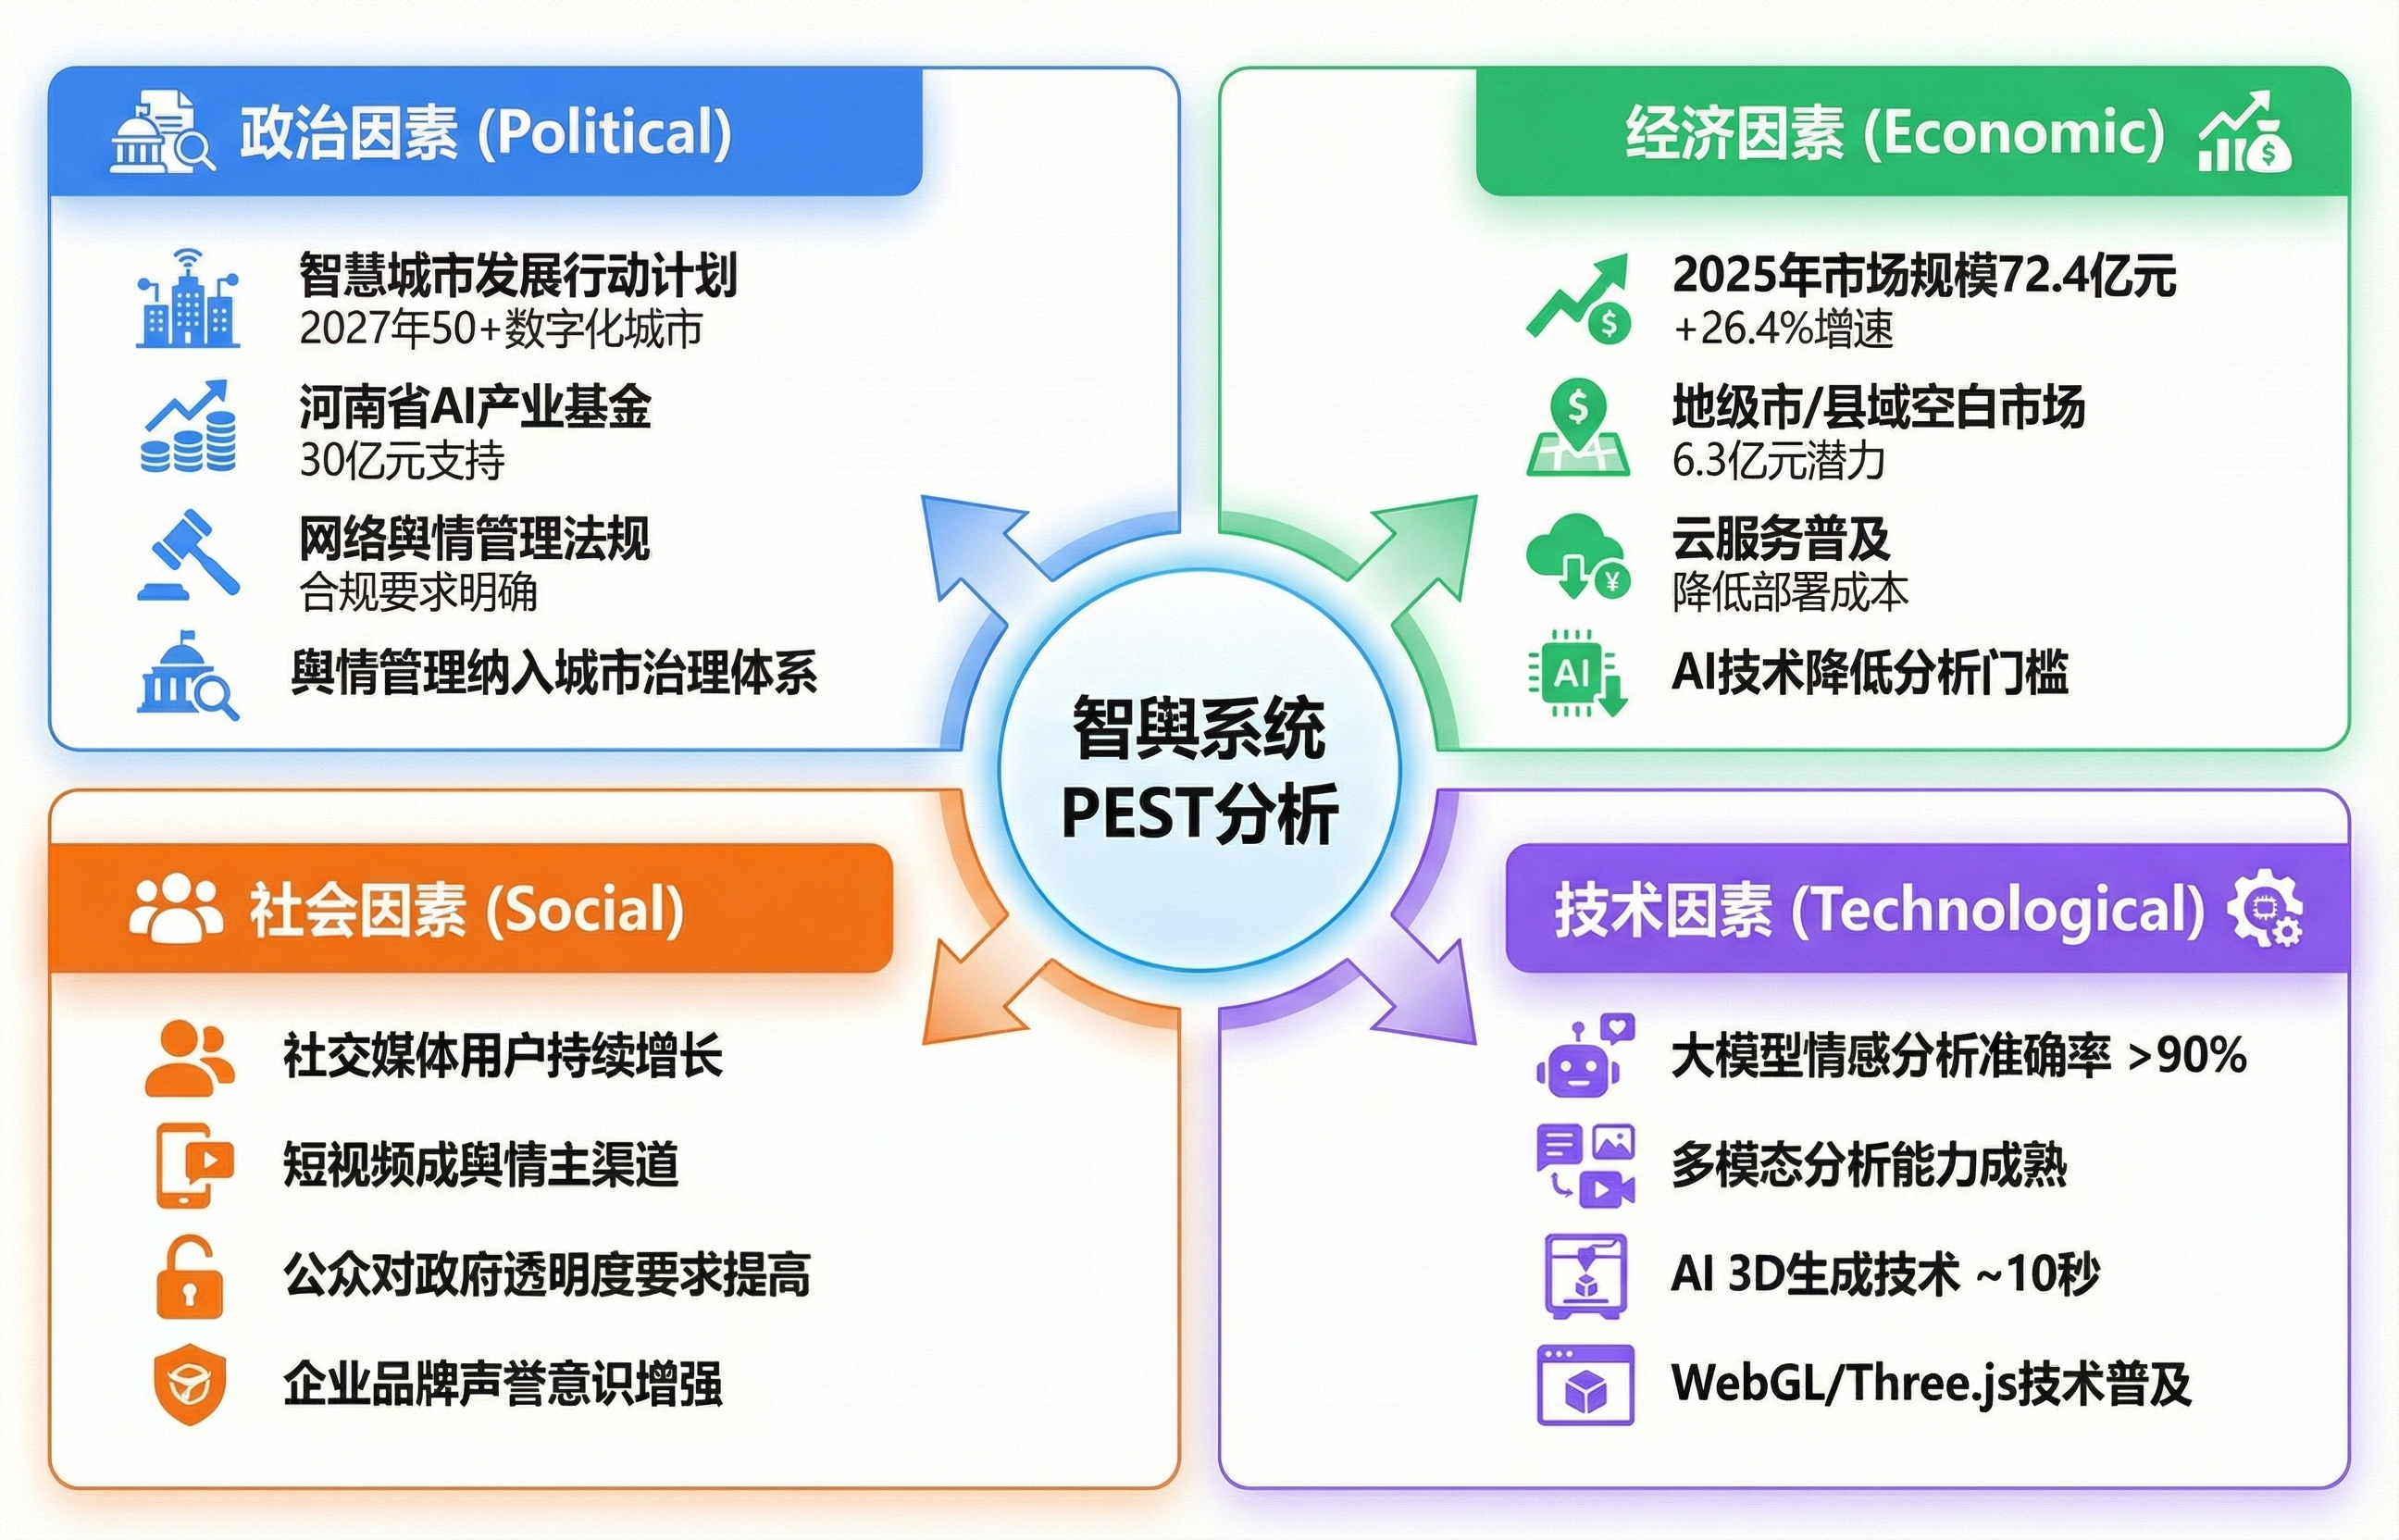
\includegraphics[width=0.85\textwidth]{../picture/fig14_PEST.png}
\caption{PEST分析四象限图}
\end{figure}

\subsubsection{行业现状}

\textbf{市场格局}

中国舆情监测市场呈现"一超多强"格局。\textbf{第一梯队}以新浪舆情通(蜜度)为代表,综合评分96.8分,稳居行业榜首,具备数据源全面、AI分析能力强等优势。\textbf{第二梯队}包括人民网舆情、蚁坊软件(鹰眼)、清博智能等,各具特色,分别在政务渠道、多语种支持、学术研究等方面具备优势。\textbf{第三梯队}包括慧科讯业、拓尔思、TOOM等企业,在细分领域有一定竞争力。

\textbf{竞争态势}:头部企业占据市场主导地位,但存在明显的机会窗口。首先是\textbf{价格门槛高},主流产品年费3-100万元,中小客户望而却步。其次是\textbf{功能过剩},大多数客户仅需基础监测和分析功能,高端功能利用率较低。再次是\textbf{下沉市场覆盖不足},地级市、县域等基层市场缺乏适配产品。最后是\textbf{创新空间大},3D可视化、AI场景生成、决策模拟等方向尚未被充分开发,为新进入者提供了差异化竞争的机会。

\subsection{项目市场趋势}

\subsubsection{市场规模}

\textbf{全球市场}:2024年规模23.15亿美元,2031年预测40.50亿美元,年复合增长率8.1\%\textsuperscript{[5]}。

\textbf{中国市场}:2024年规模110亿元人民币,年复合增长率15-26\%。

\textbf{地级市/县域市场}:全国共有地级市293个、县级行政区2844个。假设其中10\%具有舆情监测需求,平均客单价2万元/年,则潜在市场规模为:
\[
S = (293 + 2844) \times 10\% \times 2 \approx 627 \text{(万元)} \approx 6.3 \text{(亿元)}
\]
这是一个被头部企业忽视的巨大市场,也是智舆系统重点突破的目标市场。

\begin{figure}[H]
\centering
\includegraphics[width=0.9\textwidth]{../picture/fig15_market_forecast.png}
\caption{舆情监测市场规模增长预测图(2024-2031)}
\end{figure}

\subsubsection{增长驱动因素}

舆情监测市场增长受四大因素驱动。\textbf{政策推动}方面,智慧城市、数字政府建设加速推进,各级政府对舆情监测能力建设的重视程度持续提升。\textbf{技术进步}方面,AI大模型技术的成熟大幅降低了舆情分析的技术门槛和成本。\textbf{需求释放}方面,中小企业和基层政府的舆情监测意识逐步觉醒,市场需求加速释放。\textbf{场景拓展}方面,舆情监测应用从传统的政务管理领域向企业品牌维护、个人影响力管理等新场景延伸。

\subsection{目标市场}

\subsubsection{目标用户画像}

\textbf{核心用户群:地级市政府部门}

\begin{table}[H]
\centering
\caption{核心用户画像}
\begin{tabular}{L{3cm}L{10cm}}
\toprule
\textbf{特征维度} & \textbf{描述} \\
\midrule
机构类型 & 应急管理局、网信办、公安局、宣传部等 \\
预算范围 & 5-20万元/年 \\
核心需求 & 舆情监测、预警通知、分析报告 \\
痛点 & 技术人才缺乏、预算有限、现有工具不适配 \\
决策因素 & 价格、易用性、本地化服务 \\
\bottomrule
\end{tabular}
\end{table}

\textbf{拓展用户群:地方企业}

\begin{table}[H]
\centering
\caption{拓展用户画像}
\begin{tabular}{L{3cm}L{10cm}}
\toprule
\textbf{特征维度} & \textbf{描述} \\
\midrule
企业类型 & 本地品牌企业、餐饮连锁、房地产等 \\
预算范围 & 1-5万元/年 \\
核心需求 & 品牌监测、竞品分析、危机预警 \\
痛点 & 专业工具太贵、功能太复杂 \\
决策因素 & 性价比、操作简便 \\
\bottomrule
\end{tabular}
\end{table}

\subsubsection{市场细分}

\begin{table}[H]
\centering
\caption{市场细分分析}
\begin{tabular}{L{2.5cm}C{2cm}C{2cm}C{2cm}C{2cm}}
\toprule
\textbf{细分市场} & \textbf{市场规模} & \textbf{竞争强度} & \textbf{进入难度} & \textbf{优先级} \\
\midrule
信阳本地 & 小 & 低 & 低 & 高 \\
河南省内 & 中 & 中 & 中 & 中 \\
全国地级市 & 大 & 中 & 高 & 低(远期) \\
\bottomrule
\end{tabular}
\end{table}

\subsection{市场调查及分析}

\subsubsection{用户需求调研}

\textbf{政府部门需求}:$7\times24$小时不间断全网监测、多渠道预警、舆情分析功能、专项服务保障。

\textbf{企业用户需求}:实时监测品牌关键词、I级危机1小时内响应、竞品动态监测、定期舆情报告。

\subsubsection{竞品分析}

\begin{table}[H]
\centering
\caption{主要竞品对比}
\begin{tabular}{L{2.5cm}C{2cm}L{2.5cm}L{2.5cm}L{2.5cm}}
\toprule
\textbf{产品} & \textbf{评分} & \textbf{价格区间} & \textbf{核心优势} & \textbf{主要不足} \\
\midrule
新浪舆情通 & 96.8 & 3-25万/年 & 数据全、AI强 & 价格高 \\
人民网舆情 & 92.3 & 5-50万/年 & 权威背书 & 定制化程度高 \\
鹰眼速读网 & 89.7 & 3-30万/年 & 多语种 & 功能复杂 \\
清博舆情 & 87.5 & 2-20万/年 & 学术支撑 & 可视化一般 \\
\bottomrule
\end{tabular}
\end{table}

\textbf{智舆系统竞争定位}:差异化定位聚焦下沉市场,提供轻量化、低成本方案;3D可视化、AI生成、决策模拟形成差异化壁垒;立足信阳,深耕本地需求。

\begin{figure}[H]
\centering
\includegraphics[width=0.8\textwidth]{../picture/fig16.png}
\caption{竞品功能对比雷达图}
\end{figure}

% 第五章 项目营销策略
\section{项目营销策略}

\subsection{项目营销目标}

\subsubsection{短期目标(1年内)}

项目首年的核心目标是完成产品MVP开发并实现本地市场突破。具体而言,需完成系统核心功能开发并上线运行,在信阳本地获取3-5个试点客户(包括政府部门和本地企业),通过参加2-3个创新创业大赛获得行业曝光和品牌背书,积累首批成功案例为后续推广奠定基础。

\subsubsection{中期目标(1-3年)}

中期目标是实现省内市场扩张和商业模式验证。计划将业务扩展至河南省内10个主要地级市(郑州、洛阳、开封等),付费客户数突破50家,年收入突破50万元。同时建立本地化服务团队,形成销售、实施、售后的完整服务体系。

\subsubsection{长期目标(3-5年)}

长期目标是成为下沉市场舆情监测领域的头部品牌。计划覆盖全国主要地级市市场,付费客户数达到500家,年收入突破500万元,并建立起广泛的合作伙伴网络,形成可持续的竞争壁垒。

\subsection{项目营销活动}

\subsubsection{品牌建设}

品牌建设采取多渠道策略。首先通过参加创新创业大赛获得奖项背书和媒体曝光,提升品牌可信度。其次通过技术内容输出在CSDN、掘金等开发者社区分享技术文章,建立技术影响力。同时制作案例视频录制产品演示和客户案例视频,投放B站、抖音等平台,扩大产品知名度。

\subsubsection{获客渠道}

获客采取线上线下结合的方式。\textbf{政府对接}方面,通过学校产学研合作资源对接本地政府部门,争取试点合作机会。\textbf{企业拜访}方面,主动走访本地龙头企业,进行需求调研和产品推介。\textbf{线上获客}方面,通过官网、微信公众号、小程序等渠道持续获取潜在客户线索。

\subsubsection{客户运营}

客户运营注重全生命周期管理。在获客阶段,提供\textbf{14天免费试用}降低决策门槛。在上手阶段,提供\textbf{专业培训支持}包括产品培训视频、操作指南、专属客服等。在使用阶段,\textbf{定期回访}收集客户反馈并持续优化产品,确保客户成功。

\subsection{项目发展策略}

\subsubsection{产品策略}

\textbf{版本规划}

\begin{table}[H]
\centering
\caption{产品版本规划}
\begin{tabular}{L{2cm}L{3cm}L{5cm}L{3cm}}
\toprule
\textbf{版本} & \textbf{目标客户} & \textbf{核心功能} & \textbf{定价} \\
\midrule
免费版 & 个人/学生 & 基础监测、简单分析 & 免费 \\
专业版 & 中小企业 & 全功能、有限额度 & 9800元/年 \\
企业版 & 大型企业/政府 & 全功能、无限额度、定制服务 & 29800元/年 \\
\bottomrule
\end{tabular}
\end{table}

\textbf{迭代策略}:采用敏捷开发模式,快速迭代;优先实现客户反馈的高频需求;持续跟进AI技术发展,保持技术领先。

\subsubsection{区域策略}

\begin{table}[H]
\centering
\caption{区域拓展策略}
\begin{tabular}{L{2.5cm}L{2cm}L{8cm}}
\toprule
\textbf{阶段} & \textbf{时间} & \textbf{目标} \\
\midrule
Phase 1 & 第1年 & 信阳本地:聚焦信阳市及下辖县区,建立标杆案例 \\
Phase 2 & 第2年 & 河南省内:扩展至郑州、洛阳等省内主要城市 \\
Phase 3 & 第3年 & 周边省份:辐射湖北、安徽、陕西等邻近省份 \\
Phase 4 & 第4-5年 & 全国市场:覆盖全国主要地级市市场 \\
\bottomrule
\end{tabular}
\end{table}

\subsection{项目推广策略}

\subsubsection{线上推广}

线上推广构建完整的数字营销体系。\textbf{官方网站}作为产品展示核心阵地,全面呈现功能特性、客户案例、价格方案等信息。\textbf{内容营销}通过技术博客、行业白皮书、舆情分析报告等专业内容吸引目标客户。\textbf{社交媒体运营}通过微信公众号、抖音号定期分享舆情热点分析和产品使用技巧。\textbf{SEO优化}针对"舆情监测""政务舆情"等关键词进行搜索引擎优化,获取持续的自然流量。

\subsubsection{线下推广}

线下推广重点突破政企客户。\textbf{大赛路演}通过参加数智讯飞杯等创新创业大赛获得展示机会和媒体曝光。\textbf{行业会议}积极参加数字政府、智慧城市相关行业会议,拓展人脉资源。\textbf{客户拜访}主动拜访市县级政府部门和本地龙头企业,进行面对面的产品演示。\textbf{合作伙伴}与本地IT服务商、系统集成商建立渠道合作关系,借力拓展市场。

\subsubsection{口碑传播}

口碑传播是最有效的营销方式。\textbf{客户案例}积累高质量成功案例,形成可复制的标杆案例库。\textbf{老带新激励}设置老客户推荐奖励机制,推荐新客户可获得1-3个月服务延期。\textbf{行业评测}主动对接行业媒体和评测机构,争取产品评测和排名推荐,提升品牌公信力。

\begin{figure}[H]
\centering
\includegraphics[width=0.85\textwidth]{../picture/fig17.png}
\caption{营销渠道矩阵图}
\end{figure}

% 附录
\newpage
\appendix
\section*{附录}
\addcontentsline{toc}{section}{附录}

\subsection*{附录A:讯飞技术应用说明}
\addcontentsline{toc}{subsection}{附录A:讯飞技术应用说明}

本项目深度集成科大讯飞多项核心技术:

\begin{table}[H]
\centering
\caption{讯飞技术应用说明}
\begin{tabular}{L{3.5cm}L{5cm}L{4.5cm}}
\toprule
\textbf{技术名称} & \textbf{应用场景} & \textbf{集成方式} \\
\midrule
讯飞星火4.0 Ultra & 舆情分析、趋势预测、决策生成 & REST API \\
讯飞星火Lite & 日常对话、轻量任务 & REST API \\
讯飞在线TTS & 语音预警播报 & WebSocket \\
讯飞实时ASR & 语音指令输入 & WebSocket \\
讯飞LFASR & 视频音频转写 & HTTP \\
讯飞NLP & 情感分析、关键词提取 & REST API \\
\bottomrule
\end{tabular}
\end{table}

\subsection*{附录C:团队成员分工}
\addcontentsline{toc}{subsection}{附录C:团队成员分工}

\begin{table}[H]
\centering
\caption{团队成员分工}
\begin{tabular}{L{3cm}L{3cm}L{7cm}}
\toprule
\textbf{成员} & \textbf{角色} & \textbf{主要职责} \\
\midrule
{安思言} & 项目负责人 & 项目管理、产品设计、文档撰写  前端开发  Vue3开发、地图可视化、UI实现 \\
{李智康} & 后端开发 & API开发、数据库设计、系统架构 \\
{叶照扬} & 策划书 & \\
{王佳蕾} & PPT &  \\
{李欣然} & PPT &  \\
{程文飞} & 演讲 &  \\
\bottomrule
\end{tabular}
\end{table}

\subsection*{附录D:参考文献}
\addcontentsline{toc}{subsection}{附录D:参考文献}

\begin{enumerate}[leftmargin=2em]
    \item 国家发改委等五部门.《深化智慧城市发展推进全域数字化转型行动计划》.2025.10
    \item 国务院.《关于加强数字政府建设的指导意见》.2022.06
    \item 河南省人民政府.《河南省支持人工智能产业生态发展若干政策措施》.2025.08
    \item 信阳市人民政府.《信阳市数字政府建设实施方案(2023-2025年)》.2023.11
    \item QYResearch.《2024-2031全球舆情监测系统市场研究报告》.2024
    \item 蚁坊软件.《2025年中国舆情监测市场规模预测报告》.2025
    \item 拓尔思"网察"平台.《2025年舆情监测行业AI技术应用白皮书》.2025
    \item OpenAI.《GPT-5 Technical Report: Sentiment Analysis Benchmark》.2025
    \item 2025年11月舆情监测行业测评报告(新浪舆情通96.8分、人民网92.3分等).2025.11
\end{enumerate}

\vspace{2cm}

\begin{center}
\rule{0.6\textwidth}{0.4pt}

\vspace{1cm}



\end{center}


\end{document}
